% ---------------------------------------------------------------------------
% Comparison with axis-aligned learners (XGBoost, LightGBM, CatBoost) and the
% speedup map. Numbers come from benchmarks/results/spo_vs_gbt/ (drivers in
% benchmarks/evaluation/spo_vs_gbt/, protocol in /home/ubuntu/spo_vs_gbt/PROTOCOL.md).
% Tables table_spo_vs_gbt_*.tex and figures figures/results/spo_vs_gbt_* are
% generated by analyze.py -- regenerate, never hand-edit.
% ---------------------------------------------------------------------------
\subsection{Is a faster sparse oblique forest worth having? Comparison with XGBoost, LightGBM and CatBoost}
\label{sec:spo-vs-gbt}

Axis-aligned ensembles are the default choice in practice because they are cheap to train, so a
speedup of sparse oblique (SPO) training only matters if the resulting learner is competitive with
them in accuracy \emph{and} training time. We therefore compare our shipped configuration
(dynamic histogram/exact switching with vectorized binning, ``SPO Dyn-Vec'') against the
published SO-YDF exact baseline, YDF's own axis-aligned learners, and XGBoost, LightGBM and
CatBoost, in both ensemble families. All methods use 48 threads on the same machine
(Section~\ref{sec:dyn}), one training process per run, and see byte-identical training and test
matrices.

\paragraph{Protocol.}
Two families are compared \emph{within} themselves, never against each other, because they
have different capacities: random forests train 240 fully grown trees (to purity, bootstrap
sampling, $\sqrt{F}$ candidate features or projections per node), gradient boosted trees train
300 trees of depth~6 with learning rate~0.1, a minimum of five examples per leaf, no
subsampling and no early stopping. The RF family contains six SPO-YDF variants (exact with
\texttt{std::sort} as published, exact with Highway's vectorized sort, random 64-bin histograms
with scalar and vectorized binning, and the dynamic switch with scalar and vectorized binning),
YDF's axis-aligned RF, and the random-forest modes of XGBoost (\texttt{XGBRFClassifier},
unlimited depth, 63.2\% subsampling, $\sqrt{F}/F$ features per node) and LightGBM
(\texttt{boosting\_type=rf}, unlimited depth, $2^{17}$ leaves, bagging 63.2\%). The GBT family
contains SPO-GBT with exact and dynamic split finding, YDF's axis-aligned GBT (all features),
XGBoost (\texttt{hist}), LightGBM (63 leaves, \texttt{min\_child\_samples}=5) and CatBoost
(symmetric trees, bootstrap disabled). Histogram bin counts are the libraries' defaults (64 for
SPO, 256/255/254 for XGBoost/LightGBM/CatBoost); no class weights are used anywhere. Small
and medium datasets are the 30 binary TabArena-v0.1 tasks~\cite{tabarena} (748 to 150k rows, 4 to
1776 features; categorical columns ordinal-encoded, missing values imputed with the training
fold mean) evaluated by stratified 5-fold cross-validation with identical folds for every
method, plus three TabReD~\cite{tabred} classification datasets (40k-row public mirror, 119 to 696
features) evaluated on a chronological 80/20 holdout as TabReD prescribes. Large datasets are
HIGGS (10.5M training rows, 500k test), SUSY (4.5M/500k) and Epsilon (400k/100k, 2000 features),
each a single held-out split. Training time is the learner's own training timer (bootstrap and
all trees; for the Python libraries the wall time of \texttt{fit()} on an in-memory
\texttt{float32} matrix, which includes their binning). YDF additionally spends a
single-threaded post-training pass on structural variable importances and leaf indexing
(400\,s on HIGGS RF, reported separately in Table~\ref{tab:spo-vs-gbt-huge}); the Python
libraries compute importances lazily, so this pass is excluded from every headline time. ROC
AUC is the primary metric (several suite datasets have 2--7\% positives); accuracy and
log-loss are reported alongside. Across datasets we use mean ranks with a Friedman test and
Nemenyi critical differences, and for the fixed comparisons of SPO Dyn-Vec against each
competitor a Wilcoxon signed-rank test over paired folds with Holm correction, calling a
dataset a tie when $|\Delta\mathrm{AUC}|<0.005$.


\begin{figure*}[t]
    \centering
    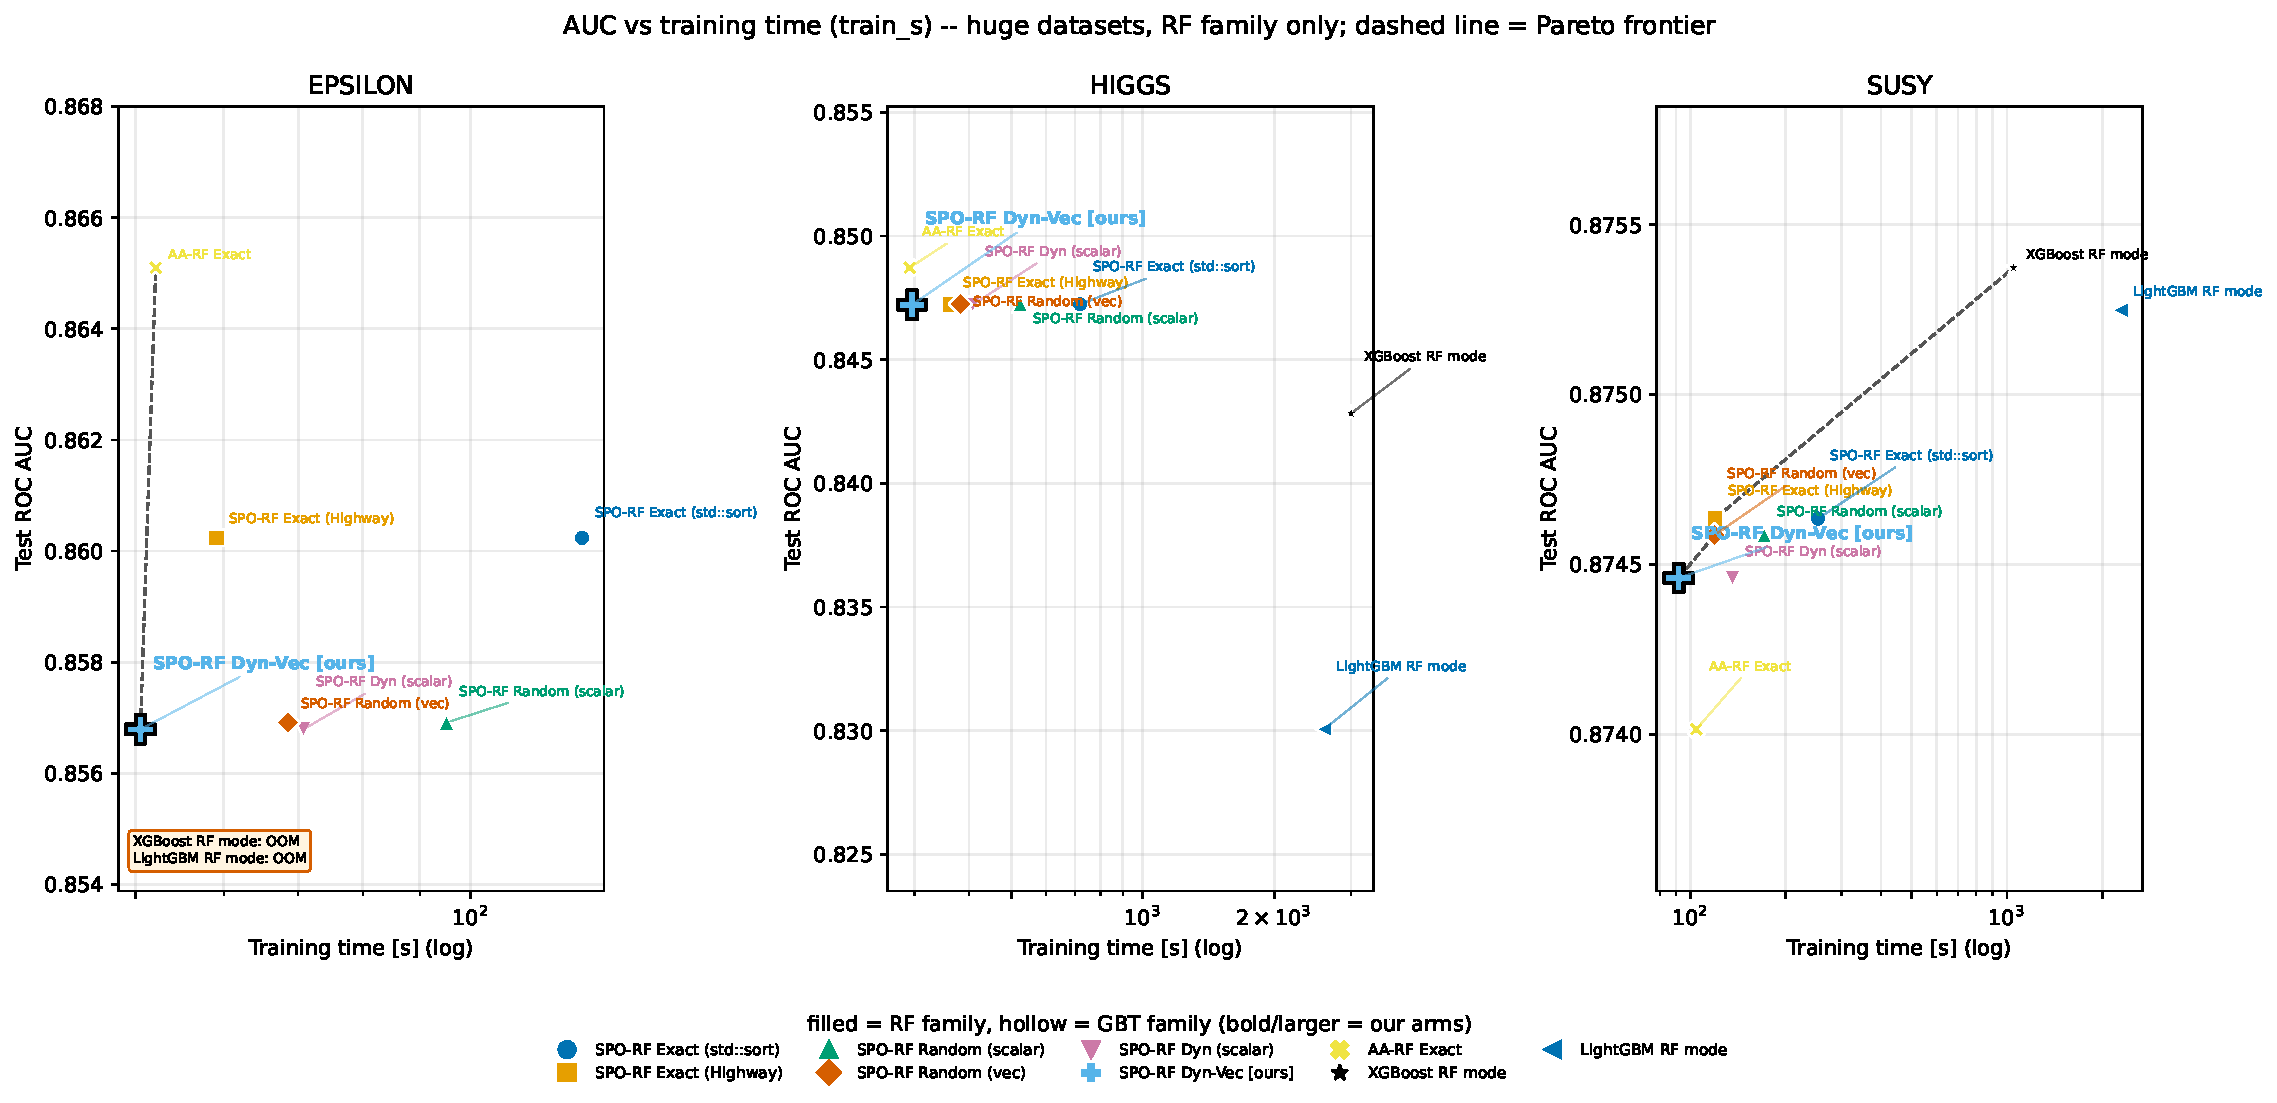
\includegraphics[width=\linewidth]{figures/results/spo_vs_gbt_pareto_rf.pdf}
    \caption{Random-forest family on the three large datasets: test ROC AUC against training time
    (log scale, 48 threads, 240 fully grown trees). Dashed line: Pareto frontier. Our SPO Dyn-Vec sits on
    the frontier of every dataset; the random-forest modes of XGBoost and LightGBM are one order of
    magnitude slower on HIGGS and SUSY and run out of memory (377\,GB) on Epsilon.}
    \Description{Three scatter panels of AUC versus training time for the RF-family learners.}
    \label{fig:spo-vs-gbt-pareto}
\end{figure*}

\begin{figure}[t]
    \centering
    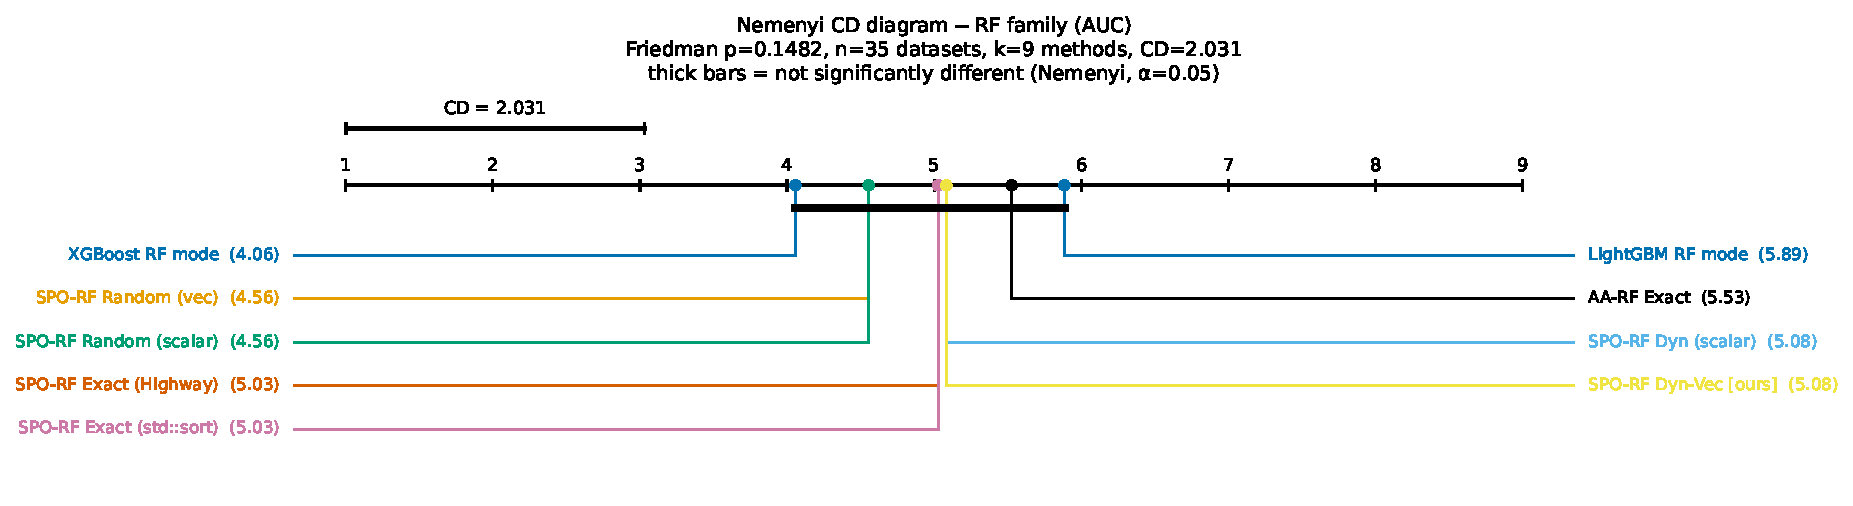
\includegraphics[width=\linewidth]{figures/results/spo_vs_gbt_cd_rf_auc.pdf}\\[4pt]
    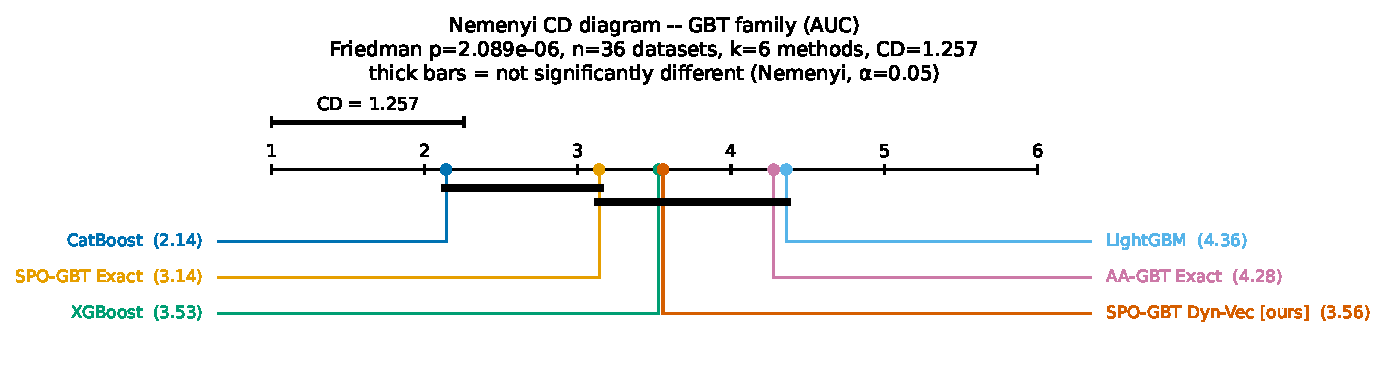
\includegraphics[width=\linewidth]{figures/results/spo_vs_gbt_cd_gbt_auc.pdf}
    \caption{Nemenyi critical-difference diagrams of mean AUC rank over the TabArena/TabReD suite
    and the three large datasets, RF family (top) and GBT family (bottom). Methods joined by a
    thick bar are not significantly different ($\alpha=0.05$).}
    \Description{Two critical-difference diagrams.}
    \label{fig:spo-vs-gbt-cd}
\end{figure}

\paragraph{Accuracy.}
Table~\ref{tab:spo-vs-gbt-summary} and Figure~\ref{fig:spo-vs-gbt-cd} summarize the suite. In
the RF family the nine learners are statistically indistinguishable (Friedman $p=0.15$ over
the 33 suite datasets plus HIGGS and SUSY; Epsilon is excluded from the RF ranking because the
library RF modes fail on it): SPO Dyn-Vec ties the SPO exact baseline on 34 of 36 datasets and
never differs from it significantly, ties XGBoost's RF mode on 15 datasets (7 wins, 13 losses,
mean $\Delta$AUC $0.005$ in XGBoost's favour) and beats LightGBM's RF mode on 11 datasets with
one loss. In the GBT family the differences are significant (Friedman $p=2\times10^{-6}$, 36
datasets): CatBoost ranks first (2.1), followed by SPO-GBT exact (3.1), XGBoost (3.5) and SPO-GBT
Dyn-Vec (3.6), ahead of axis-aligned YDF GBT (4.3) and LightGBM (4.4); SPO-GBT Dyn-Vec beats
LightGBM on 17 datasets (8 losses) and ties XGBoost on 17 (9 wins, 10 losses). No pairwise
comparison against SPO Dyn-Vec survives Holm correction,
i.e. on these datasets sparse oblique splits are as accurate as the best axis-aligned learners,
not better. On the large datasets (Table~\ref{tab:spo-vs-gbt-huge}) the picture is sharper: in
the RF family SPO Dyn-Vec reaches AUC 0.847 on HIGGS versus 0.843 for XGBoost-RF and 0.830 for
LightGBM-RF, and the two library RF modes exhaust the 377\,GB of the machine on Epsilon
(unlimited-depth trees over 2000 features); axis-aligned YDF RF is within 0.002--0.008 of SPO on
all three. In the GBT family at depth~6 the axis-aligned learners are more accurate than SPO-GBT
on HIGGS (0.825 vs 0.810) and Epsilon (0.943 vs 0.935) and tie on SUSY.

\paragraph{Training time.}
Figure~\ref{fig:spo-vs-gbt-pareto} places every learner on the accuracy--time plane of the three
large datasets. In the RF family, our work moves SPO from the slowest learner to the fastest: on
HIGGS the published SO-YDF exact baseline needs 719\,s, SPO Dyn-Vec 296\,s ($2.4\times$; the
vectorized sort alone accounts for 719$\to$363\,s and the dynamic vectorized histograms for
363$\to$296\,s), YDF's axis-aligned RF 292\,s, XGBoost's RF mode 3001\,s and LightGBM's RF mode
2599\,s---a $10\times$ and $8.8\times$ advantage for SPO at higher AUC. The same ordering holds
on SUSY (253$\to$92\,s for SPO, 104\,s axis-aligned, 1049\,s XGBoost-RF, 2281\,s LightGBM-RF) and
Epsilon (126$\to$51\,s, 52\,s axis-aligned, both library RF modes out of memory). Large-dataset
times are the median of two runs; repeats agree within 3\% for every YDF arm. Fully grown
forests are simply not what the boosting libraries are engineered for, and it is this regime
that sparse oblique forests, and the biomedical applications that motivate them, require. In
the GBT family the reverse is true: at depth~6 XGBoost and LightGBM train HIGGS in
18--22\,s and SUSY in 6--7\,s, CatBoost in 36 and 15\,s, while SPO-GBT Dyn-Vec needs 1242 and
461\,s (the SPO exact baseline 1618 and 638\,s; axis-aligned YDF GBT 747 and 268\,s). Shallow
trees over millions of rows are dominated by the per-node histogram construction over all rows,
where the libraries' pre-binned, histogram-subtracting, feature-parallel kernels cannot be
matched by per-node projections that must re-gather every row; our dynamic switch never fires
at depth~6 and vectorized binning is the only contribution that applies (1.3$\times$ on HIGGS,
1.4$\times$ on SUSY). On the wide Epsilon the gap closes (SPO-GBT 75\,s vs. 53--56\,s for
XGBoost/LightGBM and 24\,s for CatBoost) because the $\sqrt{F}$ projections per node are far
fewer than the 2000 features the axis-aligned learners must histogram. On the small suite
every learner trains in well under a minute; the per-dataset times are in the appendix
(Table~\ref{tab:spo-vs-gbt-per-dataset}).

\paragraph{Take-away.}
The answer to ``if XGBoost is sufficient, why speed up SPO?'' is that XGBoost is sufficient for
shallow boosted trees, where SPO offers no accuracy advantage and we do not claim one, but the
libraries are not an option for fully grown sparse oblique forests: their RF modes are an order
of magnitude slower than our SPO training on large datasets and fail outright on wide ones,
while our optimizations bring SPO-RF to the training time of an axis-aligned random forest at
equal or better accuracy.

\subsection{Where the speedup comes from: dataset size, depth, width and stopping criterion}
\label{sec:speedup-map}

Figure~\ref{fig:speedup-map} maps the end-to-end speedup of SPO Dyn-Vec over the two exact
baselines along the four axes a practitioner controls. \textbf{Depth} (HIGGS, 10.5M rows, 240
trees): against exact splitting with Highway's vectorized sort the speedup is $1.78\times$ at
depth~6, $1.57\times$ at 10, $1.42\times$ at 15, $1.35\times$ at 20 and $1.22\times$ for fully
grown trees; against the published \texttt{std::sort} baseline it is $2.42\times$ at full depth.
Shallow trees consist only of large nodes, where every split is found by the vectorized
histogram, so the histogram contribution is largest there; as depth grows the exact finder takes
over for the millions of small nodes and both arms converge, which is exactly the regime the
dynamic switch was designed for---without it the histogram-only arm is slower than exact at
full depth (382\,s vs 363\,s on HIGGS, Table~\ref{tab:spo-vs-gbt-huge}).
\textbf{Stopping criterion}: raising the minimum node size from 1 to 5, 20 and 100 examples
removes the smallest nodes and raises the full-depth speedup from $1.22\times$ to $1.23$,
$1.27$ and $1.31\times$. \textbf{Width} (Trunk, 1M rows, full depth): from 32 to 8192
features the speedup over \texttt{std::sort} decreases only from $3.1\times$ to $2.4\times$
and over the Highway sort from $1.34\times$ to $1.21\times$, because width enters only through
the number of projections per node ($\lceil\sqrt{F}\rceil$) and leaves the per-projection
split search, where our work applies, unchanged. \textbf{Boosting}: for SPO-GBT at depth~6
and 10 the gain is $1.30\times$ and $1.23\times$ on HIGGS and $1.09\times$ and $1.06\times$ on
a 150k-row dataset (GiveMeSomeCredit), and at depth~30 on the latter the two arms tie
($0.97\times$): depth-limited boosting never reaches the small-node regime, so only the
vectorized binning contributes, and its gain shrinks with the 150k-row dataset's node sizes.

\begin{figure*}[t]
    \centering
    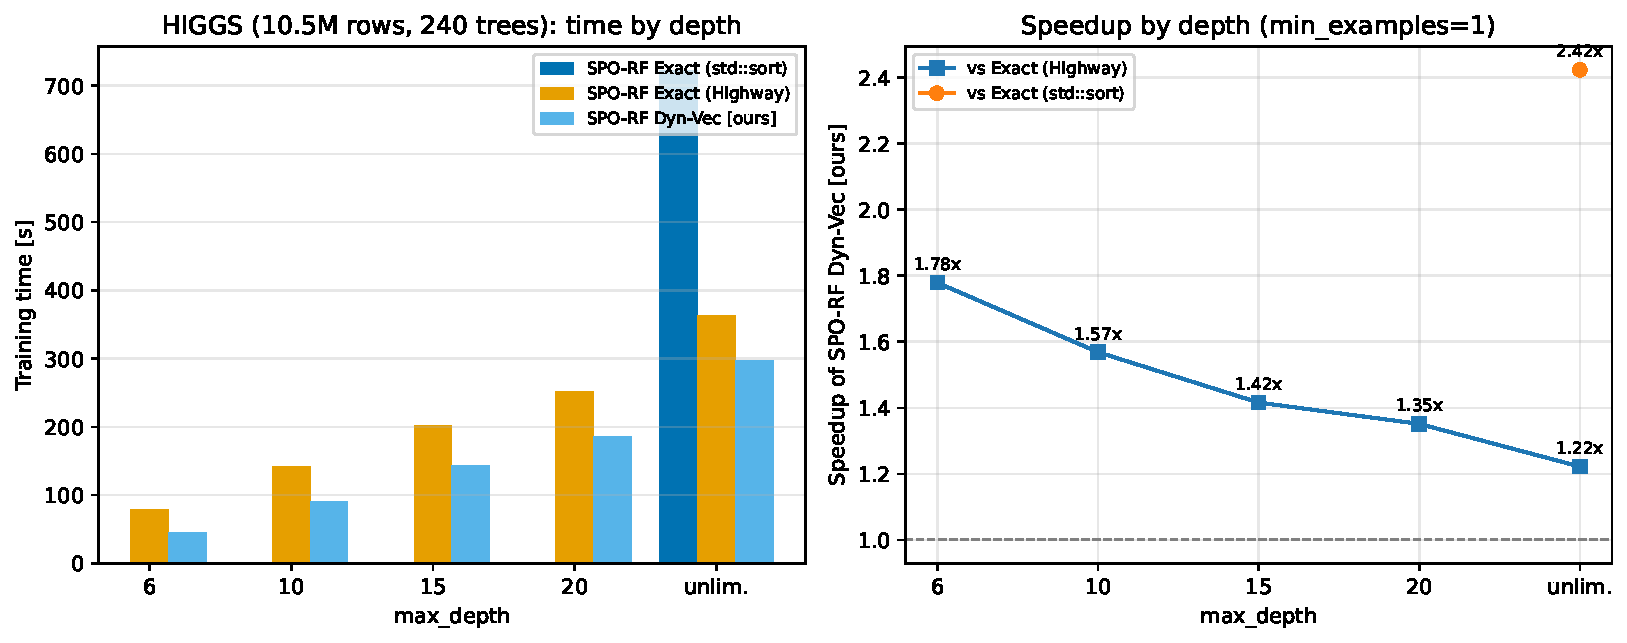
\includegraphics[width=0.49\linewidth]{figures/results/spo_vs_gbt_speedup_vs_depth.pdf}\hfill
    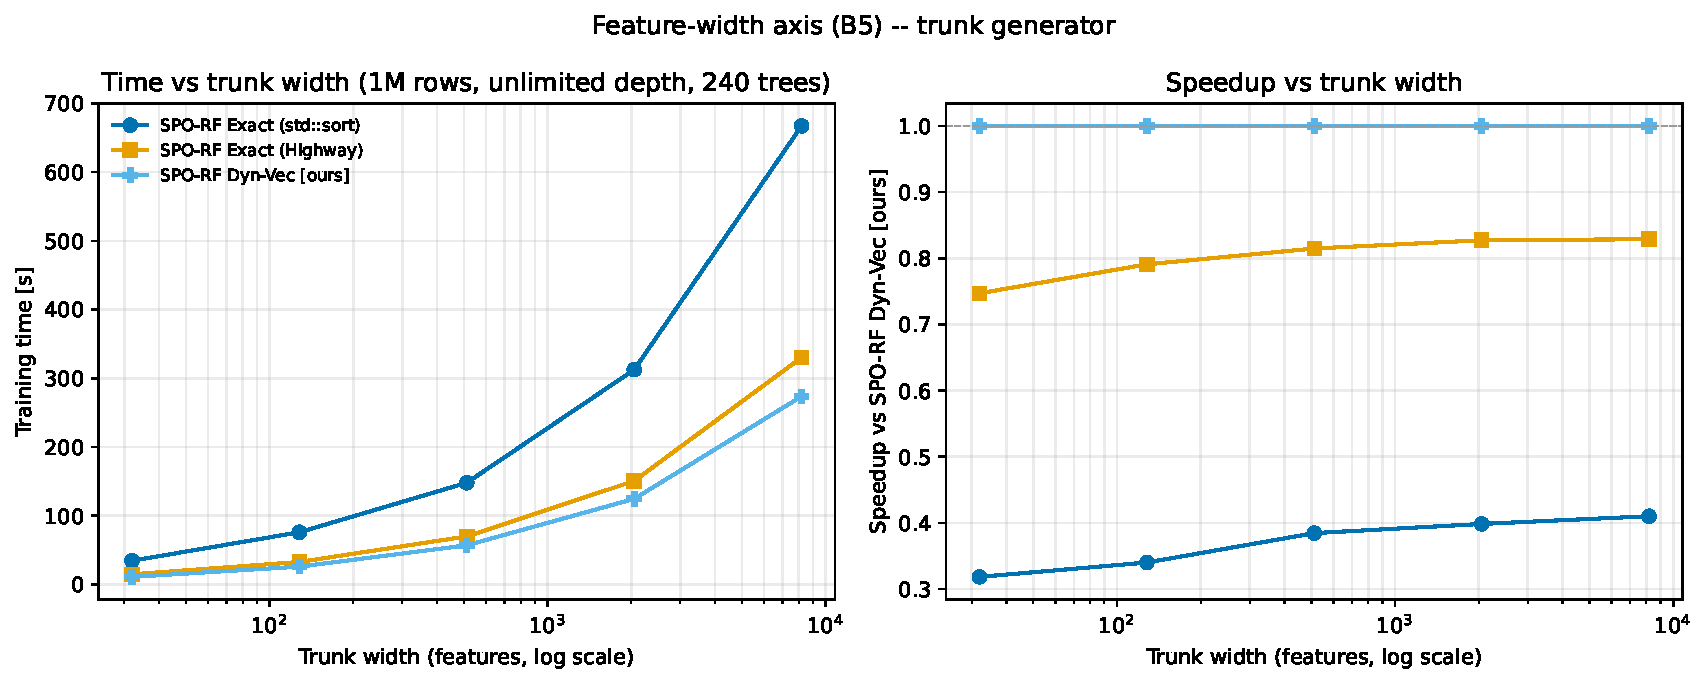
\includegraphics[width=0.49\linewidth]{figures/results/spo_vs_gbt_trunk_width.pdf}\\[4pt]
    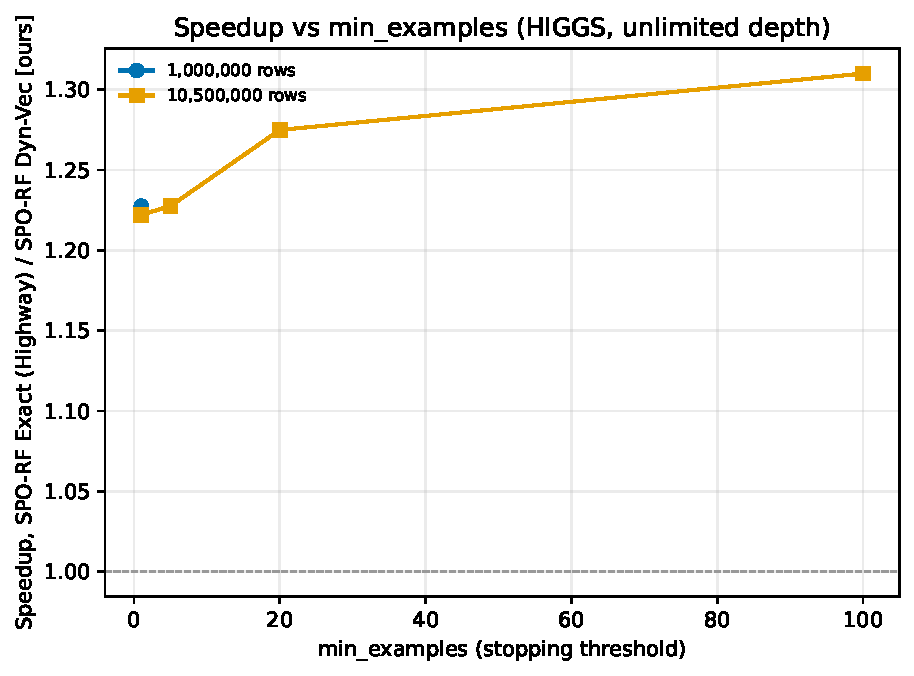
\includegraphics[width=0.49\linewidth]{figures/results/spo_vs_gbt_speedup_vs_min_examples.pdf}\hfill
    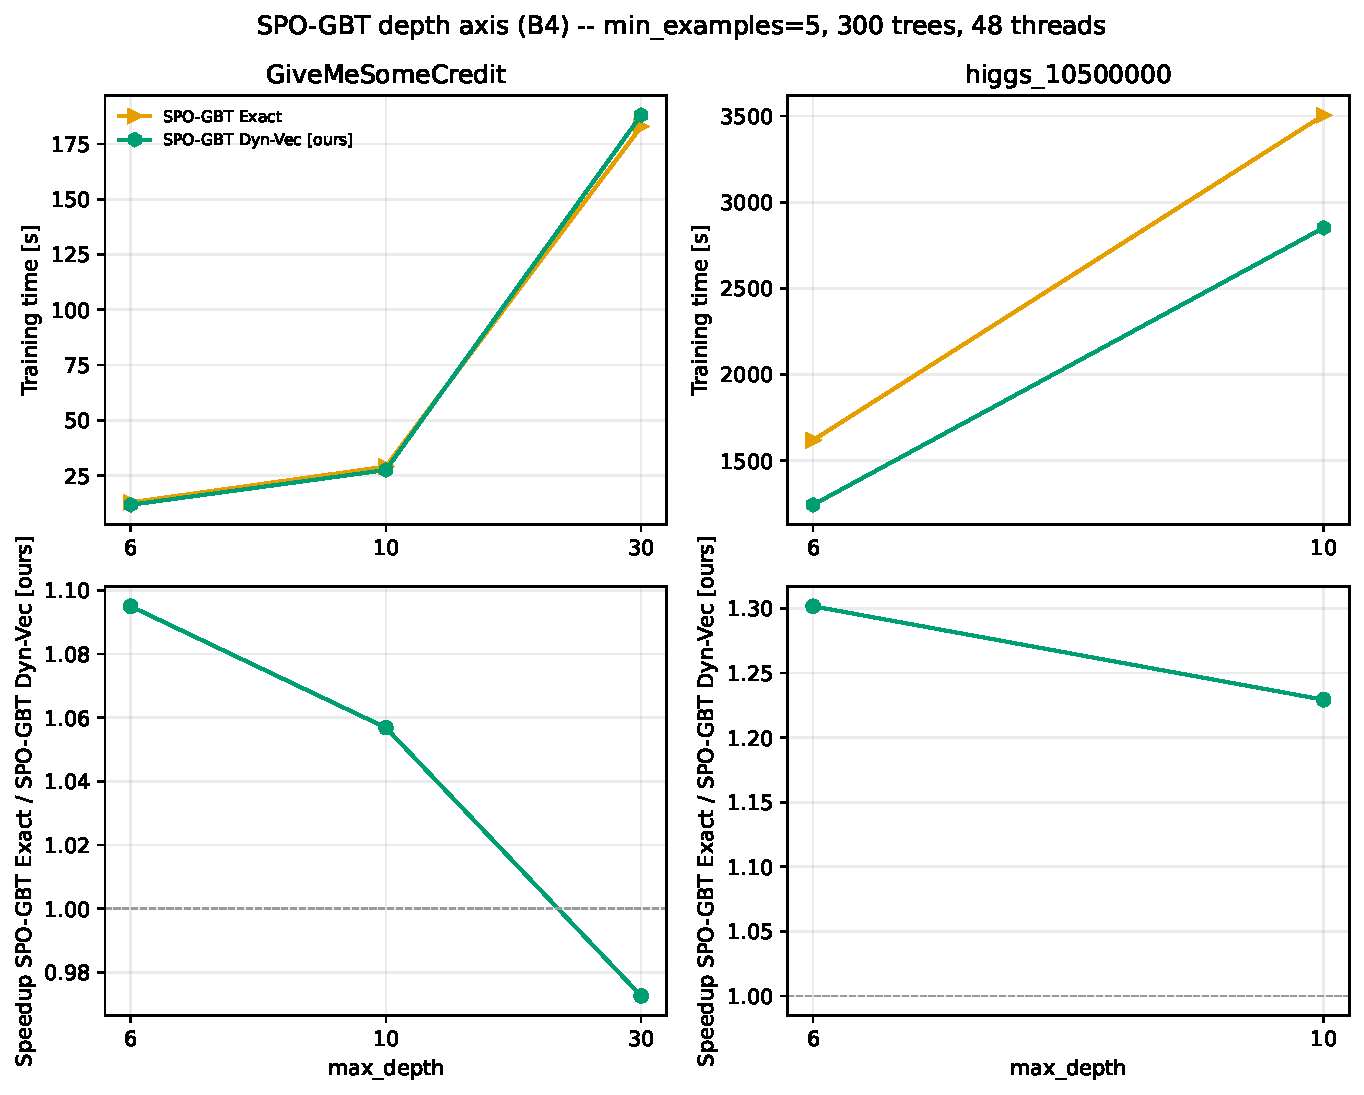
\includegraphics[width=0.49\linewidth]{figures/results/spo_vs_gbt_gbt_depth.pdf}
    \caption{Speedup map of SPO Dyn-Vec. Top left: HIGGS (10.5M rows) by maximum depth, against
    exact splitting with Highway's sort and with \texttt{std::sort}. Top right: Trunk with 1M rows by
    feature count. Bottom left: HIGGS by minimum node size. Bottom right: SPO-GBT by depth.}
    \Description{Four panels of training-time speedup along depth, width, stopping criterion and boosting depth.}
    \label{fig:speedup-map}
\end{figure*}
